Flutnings- og úthlutunarverkefni veru línuleg bestunarverkefni sem hægt er að leysa á hagkvæman máta með sérhæfðum afbrigðum af Simplex-aðferðinni sem  nýta sér sérstaka eiginleika verkefnana.
\begin{aths}Mörg hagnýt bestunarverkefni eru á þessu formi.\end{aths}

\section{Flutningsverkefni}

\ath{Flutningsverkefni} (e. transportation problem) snýst um flutning á vörum frá framleiðendum/birgjum til viðtakenda þ.a. kostnaður við að flytja vörurnar sé lágmarkaður. Látum:
\begin{enumerate}
 \item[$c_{ij}$] kostnaður við að flytja eina einingu frá $i$ til $j$.
 \item[$s_i$] framboð (e. supply) framleiðanda $i$.
 \item[$d_j$] eftirspurn (e. demand) viðtakenda $j$.
 \item[$x_{ij}$] magn sem flutt er frá $i$ til $j$.
 \item[$z$] flutningskostnaður
\end{enumerate}
G.r.f. að framboð og eftispurn sé í jafnvægi, þ.e. $\sum_i s_i = \sum_j d_j$.

\begin{daemi}[Heyflutningur] Við höfum framboð$^1$ af hey frá Vestur- og Suðurlandi ($V$ og $S$), en það er eftirspurn\footnote{tölurnar í hornklofunum} fyrir hey á Norður- og Austurlandi ($N$ og $A$).  Tölurnar við örvarnar segja svo til um kostnað per einingu:

\begin{center}
  \includegraphics[width=0.4\columnwidth]{figs/flutningsverkefni1.eps}
\end{center}
\end{daemi}

\begin{lausn}
Setjum upp í flutningstöflu þar sem framboðið kemur fram í dálki lengst til hægri og eftirspurnin í neðstu línu töflu. Fyllt er upp í töfluna með kostnaðartölum á einingu:
\[\begin{array}{|c|cc|c|}\hline 
   i / j & N\;(j=1)& A\;(j=2) & s_i \\ \hline 
  V\;(i=1) & 40 & 60 & 30 \\
  S\;(i=2) & 70 & 30 & 38 \\ \hline 
 d_j & 40  & 28 & 68 \\ \hline 
  \end{array}
\]
Þar sem $s_i$ er framboðið og $d_j$ er eftirspurnin.
\end{lausn}
Línulega bestunarverkefnið er:
$$\min_{\vec{x}} z = \sum_{i=1}^m\sum_{j=1}^n c_{ij}x_{ij}$$
Skorðurnar eru eftirfarandi jafnaðarskorður:
\begin{eqnarray*}
\sum_{j=1}^n x_{ij} &=& s_i \quad\mbox{fyrir}\quad i\in\{1,\ldots,m\}\\
\sum_{i=1}^m x_{ij} &=& d_j \quad\mbox{fyrir}\quad j\in\{1,\ldots,n\}
\end{eqnarray*}
og $x_{ij}\ge 0$ fyrir öll $i$ og $j$.

Á fylkjaformi eru skorðurnar $\vec{A}\vec{x}=\vec{b}$ með 
\begin{eqnarray*}
\begin{bmatrix}
1 & \cdots & 1 \\ & & & 1 & \cdots & 1 \\ & & & & & & \ddots \\ & & & & & & & 1 & \cdots & 1 \\ 
1 & & & 1 & & & & 1 \\
& \ddots & & & \ddots & & \cdots & & \ddots \\
& & 1 & & & 1 & & & & 1\\
 \end{bmatrix} 
\begin{bmatrix}  x_{11} \\ \vdots \\ x_{1n} \\ x_{21} \\\vdots \\ x_{2n} \\ \vdots \\ x_{m1} \\\vdots \\ x_{mn} \end{bmatrix} 
=
\begin{bmatrix}  s_1 \\ \vdots \\ s_m \\ d_1 \\\vdots \\ d_n\end{bmatrix} 
\end{eqnarray*}
Nykurverkefnið er þá
$$\max_{\vec{u},\vec{v}} w=\sum_{i=1}^m s_iu_i+\sum_{j=1}^n d_jv_j $$
m.t.t. sk.
\begin{eqnarray*}
 u_i+v_j\leq c_j \\
 u_i,\;v_j \mbox{ óskorðuð}
\end{eqnarray*}
(Skuggaverð $\vec{y}=(u_1,\ldots,u_m,v_1,\ldots,v_n)$).

\begin{aths}\hspace{.1cm}
\begin{enumerate}
\item Verkefnið hefur þann eiginleika að ef öll $s_i$ og $d_j$ eru heiltölur þá er besta lausn \emph{heiltölulausn}.
\item Það er alltaf til gjaldgeng lausn. Sjáum það með því að setja $x_{ij}=\frac{s_id_j}{K}$ þar sem $K=\sum_{i}s_i=\sum_{j}d_j$. Þá er 
$$ \sum_{j=1}^n x_{ij} = \sum_{j=1}^n \frac{s_id_j}{K}=s_i\frac{\sum_j d_j}{K}=s_i\frac{K}{K}=s_i, \quad i\in\{1,...,m\}$$
og eins fæst $\sum_{i=1}^m x_{ij}=d_j$, $j\in\{1,...,n\}$, þ.e. allar skorður uppfylltar.
%\item Til að hægt sé að uppfylla eftirspurn þarf $\sum_{i=1}^ms_i \ge \sum_{j=1}^nd_j$. 
\newpage
\begin{samepage}
\item Við reiknum með að $\sum_{i=1}^ms_i=\sum_{j=1}^nd_j$. Til að tryggja að það gangi alltaf upp þarf ef til vill að bæta við:
\begin{itemize}
  \item \ath{Gervi upphafstaður} (e. dummy source) ef $\sum s_i<\sum d_j$ með engan flutnings\-kostnað. Líka notað þegar eftirspurn er ótakmörkuð.
  \item \ath{Gervi áfangastaður} (e. dummy destination) ef $\sum s_i>\sum d_j$. %Setjum  með flutnings\-kostnað er mjög hár (stórt $M$). 
Setjum eftirspurn hjá þessum viðtakendum jafna umframboðinu og tilsvarandi kostnað sem núll.
\end{itemize} \end{samepage}
\item Ef einhver flutningsleið er ekki leyfileg má setja stóran kostnað fyrir þá leið (samsvarar stóru-$M$ aðferð). Sjá nánar bls. 313--317 í H\&L
\item Fylkið $\vec{A}$ hefur línulega háðar línur og einni skorðu er ofaukið. Þar af leiðandi er fjöldi grunnbreyta $n+m-1$.
\end{enumerate} 
\end{aths}

\section{Flutnings-Simplex aðferðin}
\ath{Flutnings-Simplex aðferðin} er löguð að stikum verkefnisins -- nýtir sér rýrleika $\vec{A}$.
\begin{description}
 \item[Fasi 1] Finna gjaldgenga grunnlausn  (alltaf til) t.d. með:
\begin{itemize}
 \item Norð-vestur aðferð
 \item Aðferð lægsta kostnaðar 
 \item Reglu Vogel
 \item Reglu Russel
\end{itemize}
\begin{samepage}
 \item[Fasi 2] Bestun
 \begin{enumerate}[label=Skref \arabic{*}]
  \item\label{flsimplex:itrun}Reikna skuggaverð $u_i,v_j$ fyrir öll $(i,j)$ sem eru í \emph{grunni}. Um grunnbreytur gildir $c_{ij}-u_i-v_j=0$.
 \item Reikna \ath{fallverð} (e. reduced cost) $r_{ij}=c_{ij}-u_i-v_j$ fyrir öll $(i,j)$ sem eru \emph{ekki í grunni}. 

Parið $(i,j)$ sem svarar til mest neikvæða gildisins á $r_{ij}$ kemur næst inn í grunn (þannig minnkar kostnaðarfallið hraðast). 

Ef öll $r_{ij}\geq0$ þá er besta lausn fundin.
 \item Ákvarða breytu sem fer úr grunni m.þ.a. finna \ath{hringrás} (e. chain reaction)
 \item Aftur í \ref{flsimplex:itrun}
 \end{enumerate}
\end{samepage}
\end{description}


%\section{Flutningstafla með kostnaði}
Dæmi \ref{daemi:flutningur} sýnir flutningstöflu þar sem kostnaður er einnig tekinn til greina. Kostnaðurinn við að senda á milli viðkomandi áfangastaða er settur í horn hvers dálks. Í upphafi þarf að finna löglega lausn. Til eru nokkrar aðferðir til að finna upphafsgrunnlausn fyrir flutningsverkefnið.

\begin{daemi}\label{daemi:flutningur}Höfum eftirfarandi kostnaðartöflu fyrir flutningsverkefni á milli verksmiðja og áfangastaða gefna 
\[ \begin{array}{cccr|cr|crcc}
 & & \multicolumn{6}{c}{\mbox{Áfangastaðir}} \\ \cline{3-8}
 & & \multicolumn{2}{|c|}{1} & \multicolumn{2}{|c|}{2} & \multicolumn{2}{|c|}{3} & s_i \\ \cline{2-9}
\multicolumn{1}{c|}{\multirow{4}{*}{\begin{sideways}Verksmiðjur\end{sideways}}} 
& \multicolumn{1}{|c|}{\multirow{2}{*}{1}} &   & \scriptscriptstyle{\fbox{10}}&    & \scriptscriptstyle{\fbox{15}} & & \scriptscriptstyle{\fbox{12}} & \multicolumn{1}{|c|}{\multirow{2}{*}{15}} \\ 
& \multicolumn{1}{|c|}{                  } &  &    &  &    & &    & \multicolumn{1}{|c|}{}\\ \cline{2-9}
& \multicolumn{1}{|c|}{\multirow{2}{*}{1}} &   & \scriptscriptstyle{\fbox{8}}&    & \scriptscriptstyle{\fbox{17}} &  & \scriptscriptstyle{\fbox{14}} & \multicolumn{1}{|c|}{\multirow{2}{*}{20}} \\ 
& \multicolumn{1}{|c|}{                  } &   &    &  &    & &    & \multicolumn{1}{|c|}{}\\ \cline{2-9}
&  \multicolumn{1}{c|}{d_j}& \multicolumn{2}{|c|}{5} & \multicolumn{2}{|c|}{18} & \multicolumn{2}{|c|}{12} & \\ \cline{3-8}
\end{array}
\]
\end{daemi}
\subsection{\ath{Norðvestur-horns} (NV) aðferðin}
\begin{enumerate}
\item Byrjum í norð-vestur horni töflunnar (efst til vinstri). 
\item Finnum lágmark á framboði og eftirspurn. % (í þessu tilviki er það eftirspurnin). 
\item Skrifum lágmarkið í stóra kassann.% (í þessu tilviki er fyrsta lágmarkið 5). 
\item Förum til hægri og finnum það lágmark sem uppfyllur skilyrði þess dálks. % (hér: höfum framboð upp á 15, búin að nýta 5 eigum því 10 eftir). 
\item Þegar öll skilyrði viðkomandi línu eru uppfyllt, förum við neðar í töfluna og endurtökum leikinn.
\begin{aths}Passa að fara alltaf til hægri þar til summan í viðkomandi línu er uppfyllt.\end{aths}
\end{enumerate}


\begin{samepage}
\begin{lausn}[á dæmi \ref{daemi:flutningur}] Notum NV-aðferðina til að finna upphafslausn:
\begin{center}
\[ \begin{array}{cccr|cr|crcc}
 & & \multicolumn{6}{c}{\mbox{Áfangastaðir}} \\ \cline{3-8}
 & & \multicolumn{2}{|c|}{1} & \multicolumn{2}{|c|}{2} & \multicolumn{2}{|c|}{3} & s_i \\ \cline{2-9}
\multicolumn{1}{c|}{\multirow{4}{*}{\begin{sideways}Verksmiðjur\end{sideways}}} 
& \multicolumn{1}{|c|}{\multirow{2}{*}{1}} &   & \scriptscriptstyle{\fbox{10}}&    & \scriptscriptstyle{\fbox{15}} & & \scriptscriptstyle{\fbox{12}} & \multicolumn{1}{|c|}{\multirow{2}{*}{15}} \\ 
& \multicolumn{1}{|c|}{                  } & \pscirclebox{5} &    & \pscirclebox{10} &    & &    & \multicolumn{1}{|c|}{}\\ \cline{2-9}
& \multicolumn{1}{|c|}{\multirow{2}{*}{2}} &   & \scriptscriptstyle{\fbox{8}}&    & \scriptscriptstyle{\fbox{17}} &  & \scriptscriptstyle{\fbox{14}} & \multicolumn{1}{|c|}{\multirow{2}{*}{20}} \\ 
& \multicolumn{1}{|c|}{                  } &   &    & \pscirclebox{8} &    & \pscirclebox{12}&    & \multicolumn{1}{|c|}{}\\ \cline{2-9}
&  \multicolumn{1}{c|}{d_j}& \multicolumn{2}{|c|}{5} & \multicolumn{2}{|c|}{18} & \multicolumn{2}{|c|}{12} & \\ \cline{3-8}
\end{array}
\]
\end{center}
\end{lausn}
\end{samepage}

\subsection{Flutningasimplex aðferðin}
\begin{enumerate}
\item Finnum gjaldgenga grunnlausn (e. BFS) með $NV$-hornsreglu,
  Vogels\-reglu eða Russelsreglu. Ef  $$\sum_{i=1}^ms_i=\sum_{j=1}^nd_j$$ þá er til leyfileg lausn.
\item Reiknum skuggaverð. Leysum
  $\vec{y}\mat{B} = \vec{c}_B$. Lát $\vec{y} = (\vec{u}_{1\times
  n}, \vec{v}_{1\times m})$ þá gildir að $u_i+v_j=c_{ij}$ fyrir
  öll $(i,j)$ í grunni (e. basic). 
 \begin{aths} Dæmigerður dálkur í $\mat{B}$ fylki  (sæti $i$ og $m+j$ með $1$ annars $0$): {\footnotesize 
$$[ u_1, u_2, \ldots, u_m, v_1, v_2, \ldots, v_n] [0, \ldots, 0, 1, 0, \ldots, 0, 1, 0, \ldots, 0]^{\text{T}} = c_{ij}$$}  
 \end{aths}

\item Finnum stak $(\hat{i},\hat{j})$ sem kemur inn í grunn. Reiknum kostnaðarminnkun
  $$\hat{c}_{ij}=c_{ij}-\vec{y}\vec{a}_{ij}$$
  þar sem $\vec{a}_{ij}$ er $(ij)$-dálkur $\mat{A}$, %)\footnote{Munið eftir lokasimplextöflunni!}.
  fyrir öll $(i,j)$ sem eru utan grunns. 

  Veljum nú það par sem gefur mesta neikvæða gildi  (þá minnkar kostn\-aðar\-fallið hraðast). Ef öll $\hat{c}_{ij}\ge 0$ er besta lausnin fundin.

\item Ákvörðum breytu sem fer úr grunni með því að finna hringrás
\begin{aths}Fylkið í flutningaverkefnum hefur línulega háðar línur. Það þýðir að einni skorðu er í raun 
ofaukið og við getum sleppt einhverri skorðunni, en hinsvegar sakar ekki að hafa hana með. Samkvæmt þessu eru grunnbreytur $n + m - 1$. % Dæmi tekið fyrir í fyrirlestri. 
\end{aths}


\end{enumerate}

\begin{daemi}\label{daemi:vorusmabilar}Flutningur úr vörubílum ($m=3$) til smásala ($n=4$).
\[ \begin{array}{cccr|cr|cr|crcc}
 & & \multicolumn{8}{c}{\mbox{Smásalar}} \\ \cline{3-10}
 & & \multicolumn{2}{|c|}{S1} & \multicolumn{2}{|c|}{S2} & \multicolumn{2}{|c|}{S3}& \multicolumn{2}{|c|}{S4} & s_i \\ \cline{2-11}
\multicolumn{1}{c|}{\multirow{6}{*}{\begin{sideways}Vöruhús\end{sideways}}} 
& \multicolumn{1}{|c|}{\multirow{2}{*}{V1}} &   & \scriptscriptstyle{\fbox{12}}&    & \scriptscriptstyle{\fbox{13}} & & \scriptscriptstyle{\fbox{4}}& & \scriptscriptstyle{\fbox{6}} & \multicolumn{1}{|c|}{\multirow{2}{*}{500}}  \\ 
& \multicolumn{1}{|c|}{                  } & &    & &    & &   & & & \multicolumn{1}{|c|}{}\\ \cline{2-11}
& \multicolumn{1}{|c|}{\multirow{2}{*}{V2}} &   & \scriptscriptstyle{\fbox{6}}&    & \scriptscriptstyle{\fbox{4}} & & \scriptscriptstyle{\fbox{10}}& & \scriptscriptstyle{\fbox{11}} & \multicolumn{1}{|c|}{\multirow{2}{*}{700}}  \\ 
& \multicolumn{1}{|c|}{                  } & &    & &    & & &&   & \multicolumn{1}{|c|}{}\\ \cline{2-11}
& \multicolumn{1}{|c|}{\multirow{2}{*}{V3}} &   & \scriptscriptstyle{\fbox{10}}&    & \scriptscriptstyle{\fbox{9}} &  & \scriptscriptstyle{\fbox{12}} & & \scriptscriptstyle{\fbox{4}} & \multicolumn{1}{|c|}{\multirow{2}{*}{800}} \\ 
& \multicolumn{1}{|c|}{                  } & &    & &    & &   & & & \multicolumn{1}{|c|}{}\\ \cline{2-11}
&  \multicolumn{1}{c|}{d_j}& \multicolumn{2}{|c|}{400} & \multicolumn{2}{|c|}{900} & \multicolumn{2}{|c}{200} &\multicolumn{2}{|c|}{500} & \\ \cline{3-10}
\end{array}
\]
\end{daemi}
\begin{lausn}Framboð og eftispurn eru í jafnvægi:
\begin{eqnarray*}
 \sum_{i=1}^m s_i &=&500+700+800=2000\\
 \sum_{j=1}^n d_j &=& 400+900+200+500=2000
\end{eqnarray*}
og því ekki þörf á að bæta við gerviupphafsstöð eða -viðtakendum.

\begin{description}
 \item[Fasi 1] Norðvestur aðferð:
 \begin{enumerate}[label=(\roman{*})]
  \item Byrja með $x_{11}$ (norð-vestur horn)
  \item\label{skref:18} Úthluta eins miklu og hægt er (hér 400) og uppfæra framboð og eftispurn.
  \item Strika út línu/dálk með núll í framboð/eftirspurn.
  \item Fara aftur í skref \ref{skref:18} þangað til gjaldgeng lausn er fengin.
 \end{enumerate}

\begin{center}

\[ \begin{array}{cccr|cr|cr|crcc}
 & & \multicolumn{8}{c}{\mbox{Smásalar}} \\ \cline{3-10}
 & & \multicolumn{2}{|c|}{S1} & \multicolumn{2}{|c|}{S2} & \multicolumn{2}{|c|}{S3}& \multicolumn{2}{|c|}{S4} & s_i \\ \cline{2-11}
\multicolumn{1}{c|}{\multirow{8}{*}{\begin{sideways}Vöruhús\end{sideways}}} 
& \multicolumn{1}{|c|}{\multirow{2}{*}{V1}} &   & \scriptscriptstyle{\fbox{12}}&    & \scriptscriptstyle{\fbox{13}} & & \scriptscriptstyle{\fbox{4}}& & \scriptscriptstyle{\fbox{6}} & \multicolumn{1}{|c|}{\multirow{2}{*}{\cancel{500}\;\cancel{100}\;0}}  \\ 
& \multicolumn{1}{|c|}{                  } & \pscirclebox{400} & & \pscirclebox{100}&    & &   & & & \multicolumn{1}{|c|}{}\\ \cline{2-11}
& \multicolumn{1}{|c|}{\multirow{2}{*}{V2}} &   & \scriptscriptstyle{\fbox{6}}&    & \scriptscriptstyle{\fbox{4}} & & \scriptscriptstyle{\fbox{10}}& & \scriptscriptstyle{\fbox{11}} & \multicolumn{1}{|c|}{\multirow{2}{*}{\cancel{700}\;0}}  \\ 
& \multicolumn{1}{|c|}{                  } &  &    & \pscirclebox{700}&    & & &&   & \multicolumn{1}{|c|}{}\\ \cline{2-11}
& \multicolumn{1}{|c|}{\multirow{2}{*}{V3}} &   & \scriptscriptstyle{\fbox{10}}&    & \scriptscriptstyle{\fbox{9}} &  & \scriptscriptstyle{\fbox{12}} & & \scriptscriptstyle{\fbox{4}} & \multicolumn{1}{|c|}{\multirow{2}{*}{\cancel{800}\;\cancel{700}}} \\ 
& \multicolumn{1}{|c|}{                  } &   &    & \pscirclebox{100}&    & \pscirclebox{200}&   & \pscirclebox{500}& & \multicolumn{1}{|c|}{\multirow{2}{*}{\cancel{500}\;0}}\\ \cline{2-11}
&  \multicolumn{1}{c|}{d_j}& \multicolumn{2}{|c|}{\cancel{400}\;0} & \multicolumn{2}{|c|}{\cancel{900}\;\cancel{800}\;0} & \multicolumn{2}{|c|}{\cancel{200}\;0} &\multicolumn{2}{|c|}{\cancel{500}\;0} & \\ \cline{3-10}
\end{array}
\]
\end{center}

Sjáum að upphafslausn er $x_{11}=400,x_{12}=100,x_{22}=700$, \mbox{$x_{32}=100$}, $x_{33}=200,x_{34}=500$ og önnur $x_{ij}=0$ með markfallsgildið
\begin{eqnarray*}
z&=&\sum_{i=1}^3\sum_{j=1}^4 c_{ij}x_{ij}=% 12\cdot400 + 13\cdot100 + 4\cdot700 + 9\cdot100+ 12\cdot200+ 4\cdot500\\& =& 
14.200 
\end{eqnarray*}

\newpage
\item[Fasi 2 -- ítrun \#1]Bestun
\begin{enumerate}
 \item Skuggaverð ($c_{ij}=u_i+v_j$) fyrir grunnbreytur. Höfum $m+n$ grunn\-breytur en $m+n-1$ óháðar skorður. Getum því sett eina $=0$.
Setjum $u_3=0$ (því það kemur oftast fyrir) og leysum $c_{ij}=u_i+v_j$ og stillum upp í töflu:
 \[ \begin{matrix}
  (1,1) & 12 &=& u_1+v_1 & \Rightarrow & v_1&=&8\\
  (1,2) & 13 &=& u_1+v_2 & \Rightarrow & u_1&=&4\\
  (2,2) &  4 &=& u_2+v_2 & \Rightarrow & u_1&=&-5\\
  (3,2) &  9 &=& u_3+v_2 & \Rightarrow & v_2&=&9\\
  (3,3) & 12 &=& u_3+v_3 & \Rightarrow & v_3&=&12\\
  (3,4) &  4 &=& u_3+v_4 & \Rightarrow & v_4&=&4\\
    \end{matrix}\]
\begin{aths}Reikna þarf $u_i$ og $v_j$ í hverri ítrun.\end{aths}

\item Fallverð $r_{ij}=c_{ij}-u_i-v_j$ fyrir breytur \emph{utan} grunns (þ.e. auðir reitir).
\[\begin{matrix}   r_{21}&=&6-(-5)-8=3 &  r_{13}&=&-12  & r_{14}&=&-2\\ 
                   r_{32}&=&10+0-8=2  &   r_{23}&=&3 & r_{24}&=&12  \end{matrix}\] 
\begin{center}
\[ \begin{array}{cccr|cr|cr|crcc}
 & & \multicolumn{8}{c}{\mbox{Smásalar}} \\ \cline{3-10}
 & & \multicolumn{2}{|c|}{S1} & \multicolumn{2}{|c|}{S2} & \multicolumn{2}{|c|}{S3}& \multicolumn{2}{|c|}{S4} &  u_i \\ \cline{2-11}
\multicolumn{1}{c|}{\multirow{8}{*}{\begin{sideways}Vöruhús\end{sideways}}} 
& \multicolumn{1}{|c|}{\multirow{2}{*}{V1}} &   & \scriptscriptstyle{\fbox{12}}&    & \scriptscriptstyle{\fbox{13}} & & \scriptscriptstyle{\fbox{4}}& & \scriptscriptstyle{\fbox{6}} & \multicolumn{1}{|c|}{\multirow{2}{*}{4}}  \\ 
& \multicolumn{1}{|c|}{} & \pscirclebox{400} & & \pscirclebox{100}&    & -12 & & -2 & & \multicolumn{1}{|c|}{}\\ \cline{2-11}
& \multicolumn{1}{|c|}{\multirow{2}{*}{V2}} &   & \scriptscriptstyle{\fbox{6}}&    & \scriptscriptstyle{\fbox{4}} & & \scriptscriptstyle{\fbox{10}}& & \scriptscriptstyle{\fbox{11}} & \multicolumn{1}{|c|}{\multirow{2}{*}{-5}}  \\ 
& \multicolumn{1}{|c|}{} & 3 &    & \pscirclebox{700}&    & 3 & & 12 &   & \multicolumn{1}{|c|}{}\\ \cline{2-11}
& \multicolumn{1}{|c|}{\multirow{2}{*}{V3}} &   & \scriptscriptstyle{\fbox{10}}&    & \scriptscriptstyle{\fbox{9}} &  & \scriptscriptstyle{\fbox{12}} & & \scriptscriptstyle{\fbox{4}} & \multicolumn{1}{|c|}{\multirow{2}{*}{0}} \\ 
& \multicolumn{1}{|c|}{} & 2  &    & \pscirclebox{100}&    & \pscirclebox{200}&   & \pscirclebox{500}& & \multicolumn{1}{|c|}{\multirow{2}{*}{}}\\ \cline{2-11}
&  \multicolumn{1}{c|}{v_j}& \multicolumn{2}{|c|}{8} & \multicolumn{2}{|c|}{9} & \multicolumn{2}{|c|}{12} &\multicolumn{2}{|c|}{4} & \\ \cline{3-10}
\end{array}
\]
\end{center}
Sjáum að við erum með neikvæð fallgildi, og $r_{13}$ kemur inn í grunn.
\newpage
\item Finnum hringrás fyrir $x_{13}$, og síðan breytuna sem fer úr grunni. 
\begin{center}
 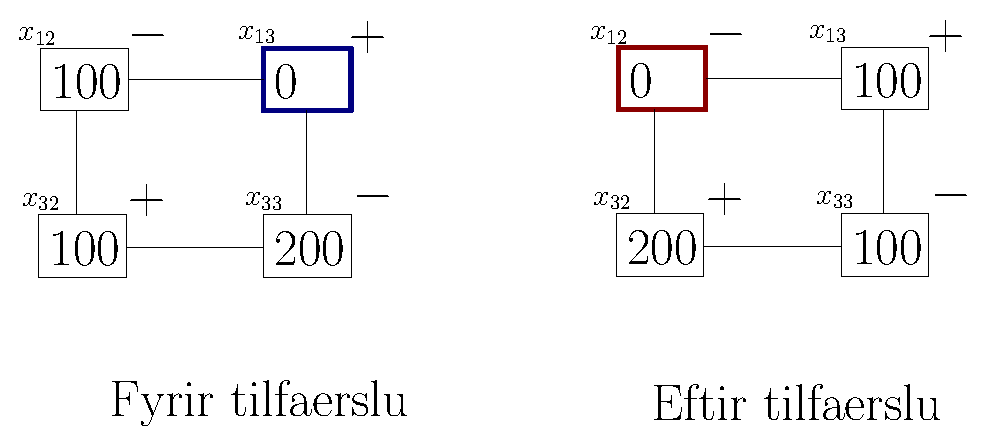
\includegraphics[width=0.6\columnwidth]{figs/flutn_bestun_hringras.eps}
\end{center}
Sjáum að $x_{12}$ fer úr grunni.
\end{enumerate}

\item[Fasi 2 -- ítrun \#2] Upphafstaflan er:
\begin{center}
\[ \begin{array}{cccr|cr|cr|crcc}
 & & \multicolumn{8}{c}{\mbox{Smásalar}} \\ \cline{3-10}
 & & \multicolumn{2}{|c|}{S1} & \multicolumn{2}{|c|}{S2} & \multicolumn{2}{|c|}{S3}& \multicolumn{2}{|c|}{S4} & s_i \\ \cline{2-11}
\multicolumn{1}{c|}{\multirow{8}{*}{\begin{sideways}Vöruhús\end{sideways}}} 
& \multicolumn{1}{|c|}{\multirow{2}{*}{V1}} &   & \scriptscriptstyle{\fbox{12}}&    & \scriptscriptstyle{\fbox{13}} & & \scriptscriptstyle{\fbox{4}}& & \scriptscriptstyle{\fbox{6}} & \multicolumn{1}{|c|}{\multirow{2}{*}{500}}  \\ 
& \multicolumn{1}{|c|}{                  } & \pscirclebox{400} & & &    &\pscirclebox{100} &   & & & \multicolumn{1}{|c|}{}\\ \cline{2-11}
& \multicolumn{1}{|c|}{\multirow{2}{*}{V2}} &   & \scriptscriptstyle{\fbox{6}}&    & \scriptscriptstyle{\fbox{4}} & & \scriptscriptstyle{\fbox{10}}& & \scriptscriptstyle{\fbox{11}} & \multicolumn{1}{|c|}{\multirow{2}{*}{700}}  \\ 
& \multicolumn{1}{|c|}{                  } &  &    & \pscirclebox{700}&    & & &&   & \multicolumn{1}{|c|}{}\\ \cline{2-11}
& \multicolumn{1}{|c|}{\multirow{2}{*}{V3}} &   & \scriptscriptstyle{\fbox{10}}&    & \scriptscriptstyle{\fbox{9}} &  & \scriptscriptstyle{\fbox{12}} & & \scriptscriptstyle{\fbox{4}} & \multicolumn{1}{|c|}{\multirow{2}{*}{800}} \\ 
& \multicolumn{1}{|c|}{                  } &   &    & \pscirclebox{200}&    & \pscirclebox{100}&   & \pscirclebox{500}& & \multicolumn{1}{|c|}{\multirow{2}{*}{}}\\ \cline{2-11}
&  \multicolumn{1}{c|}{d_j}& \multicolumn{2}{|c|}{400} & \multicolumn{2}{|c|}{900} & \multicolumn{2}{|c|}{200} &\multicolumn{2}{|c|}{500} & \\ \cline{3-10}
\end{array}
\]
\end{center}
 Síðan er haldið áfram eins og áður (gerið sjálf).
\end{description}
\end{lausn}
\newpage
\section{Gjaldgengar lausnir fyrir flutningsverkefni}
Norð-vestur aðferð horfir alveg framhjá $c_{ij}$ gildum og því getur upphafslausn verið langt frá bestu lausn sem kallar á margar ítranir í fasa 2.

\subsection{Aðferð lægsta kostnaðar}
\ath{Aðferð lægsta kostnaðar} (e. minimum cost criterion)\footnote{Sjá dæmi 8.2-4, bls. 350-1 í H\&L.} gefur yfirleitt betri upphafslausn en norð-vestur aðferð.
\begin{lausn}[á dæmi \ref{daemi:vorusmabilar}] Finnum upphafslausn með aðferð lægsta kostnaðar. 

\[ \begin{array}{cccr|cr|cr|crcc}
 & & \multicolumn{8}{c}{\mbox{Smásalar}} \\ \cline{3-10}
 & & \multicolumn{2}{|c|}{S1} & \multicolumn{2}{|c|}{S2} & \multicolumn{2}{|c|}{S3}& \multicolumn{2}{|c|}{S4} & s_i \\ \cline{2-11}
\multicolumn{1}{c|}{\multirow{8}{*}{\begin{sideways}Vöruhús\end{sideways}}} 
& \multicolumn{1}{|c|}{\multirow{2}{*}{V1}} &   & \scriptscriptstyle{\fbox{12}}&    & \scriptscriptstyle{\fbox{13}} & & \scriptscriptstyle{\fbox{4}}& & \scriptscriptstyle{\fbox{6}} & \multicolumn{1}{|c|}{\multirow{2}{*}{\cancel{500}\;\cancel{300}\;0}}  \\ 
& \multicolumn{1}{|c|}{                  } & \pscirclebox{300} &&& & \pscirclebox{200}&    & & & \multicolumn{1}{|c|}{}\\ \cline{2-11}
& \multicolumn{1}{|c|}{\multirow{2}{*}{V2}} &   & \scriptscriptstyle{\fbox{6}}&    & \scriptscriptstyle{\fbox{4}} & & \scriptscriptstyle{\fbox{10}}& & \scriptscriptstyle{\fbox{11}} & \multicolumn{1}{|c|}{\multirow{2}{*}{\cancel{700}\;0}}  \\ 
& \multicolumn{1}{|c|}{                  } &  &    & \pscirclebox{700}&    & & &&   & \multicolumn{1}{|c|}{}\\ \cline{2-11}
& \multicolumn{1}{|c|}{\multirow{2}{*}{V3}} &   & \scriptscriptstyle{\fbox{10}}&    & \scriptscriptstyle{\fbox{9}} &  & \scriptscriptstyle{\fbox{12}} & & \scriptscriptstyle{\fbox{4}} & \multicolumn{1}{|c|}{\multirow{2}{*}{\cancel{800}\;\cancel{300}}} \\ 
& \multicolumn{1}{|c|}{                  } &    \pscirclebox{100}&    & \pscirclebox{200}& &&  & \pscirclebox{500}& & \multicolumn{1}{|c|}{\multirow{2}{*}{\cancel{100}\;0}}\\ \cline{2-11}
&  \multicolumn{1}{c|}{d_j}& \multicolumn{2}{|c|}{\cancel{400}\;\cancel{300}\;0} & \multicolumn{2}{|c|}{\cancel{900}\;\cancel{200}\;0} & \multicolumn{2}{|c|}{\cancel{200}\;0} &\multicolumn{2}{|c|}{\cancel{500}\;0} & \\ \cline{3-10}
\end{array}
\]
Sjáum að $z=12000$, þ.e. finnur bestu lausn (\emph{fyrir tilviljun}) sem fæst staðfest í fasa 2.
\end{lausn}

\subsection{\ath{Aðferð Vogel}}
Fyrir sérhverja óútstrikaða línu/dálk reiknast \emph{mismunur} minnsta og næst minnsta kostnaðar. Finnum línu/dálk með mesta mismun. 
%Næsta breyta inn í grunn svarar til lægsta kostnaðar í viðkomandi\footnote{sem ekki er búið að stroka út} línu/dálki.
Veljum sem næstu grunnbreytu $x_{ij}$ sem er með minnsta óútstrikað $c_{ij}$ í línu eða dálki sem er með mesta mun. 

\begin{lausn}[á dæmi \ref{daemi:vorusmabilar}] Finnum upphafslausn með aðferð Vogels. 
\[ \begin{array}{cccr|cr|cr|crcc}
 & & \multicolumn{8}{c}{\mbox{Smásalar}} \\ \cline{3-10}
 & & \multicolumn{2}{|c|}{S1} & \multicolumn{2}{|c|}{S2} & \multicolumn{2}{|c|}{S3}& \multicolumn{2}{|c|}{S4} & s_i \\ \cline{2-11}
\multicolumn{1}{c|}{\multirow{8}{*}{\begin{sideways}Vöruhús\end{sideways}}} 
& \multicolumn{1}{|c|}{\multirow{2}{*}{V1}} &   & \scriptscriptstyle{\fbox{12}}&    & \scriptscriptstyle{\fbox{13}} & & \scriptscriptstyle{\fbox{4}}& & \scriptscriptstyle{\fbox{6}} & \multicolumn{1}{|c|}{\multirow{2}{*}{\cancel{500}\;\cancel{300}\;0}}  \\ 
& \multicolumn{1}{|c|}{                  } &&&&& \pscirclebox{200} & & \pscirclebox{300}&    & \multicolumn{1}{|c|}{}\\ \cline{2-11}
& \multicolumn{1}{|c|}{\multirow{2}{*}{V2}} &   & \scriptscriptstyle{\fbox{6}}&    & \scriptscriptstyle{\fbox{4}} & & \scriptscriptstyle{\fbox{10}}& & \scriptscriptstyle{\fbox{11}} & \multicolumn{1}{|c|}{\multirow{2}{*}{\cancel{700}\;0}}  \\ 
& \multicolumn{1}{|c|}{                  } &  &    & \pscirclebox{700}&    & & &&   & \multicolumn{1}{|c|}{}\\ \cline{2-11}
& \multicolumn{1}{|c|}{\multirow{2}{*}{V3}} &   & \scriptscriptstyle{\fbox{10}}&    & \scriptscriptstyle{\fbox{9}} &  & \scriptscriptstyle{\fbox{12}} & & \scriptscriptstyle{\fbox{4}} & \multicolumn{1}{|c|}{\multirow{2}{*}{\cancel{800}\;\cancel{600}}} \\ 
& \multicolumn{1}{|c|}{                  } &   \pscirclebox{400}&    & \pscirclebox{200}&  && & \pscirclebox{200}& & \multicolumn{1}{|c|}{\multirow{2}{*}{\cancel{400}\;0}}\\ \cline{2-11}
&  \multicolumn{1}{c|}{d_j}& \multicolumn{2}{|c|}{\cancel{400}\;0} & \multicolumn{2}{|c|}{\cancel{900}\;\cancel{200}\;0} & \multicolumn{2}{|c|}{\cancel{200}\;0} &\multicolumn{2}{|c|}{\cancel{500}\;\cancel{200}\;0} & \\ \cline{3-10}
\end{array}
\]
\vspace{5cm}

Sjáum að $z=12000$, þ.e. finnur bestu lausn (\emph{fyrir tilviljun}) sem fæst staðfest í fasa 2.
\end{lausn}




\subsection{\ath{Russel} regla}
Reiknum fyrir allar óútstrikaðar línur $i$ og dálka $j$:

$$\bar{u}_i = \max_{i\in \tiny{\mbox{ óútstr. dálkur }}}c_{ij} ~~~~~~~ \bar{v}_j = \max_{j\in \tiny{\mbox{ óútstr. lína }}}c_{ij}$$
$$\Delta_{ij}=c_{ij}-\bar{u}_i-\bar{v}_j$$
Næsta grunnbreyta er sú sem hefur minnsta $\Delta_{ij}$.

\begin{aths}Sjá dæmi á bls. 342, tafla 8.18, í H\&L. \end{aths}

\begin{daemi}[Flutningsverkefni í \athsub{\textsc{MathProg}}{\texttt{transport.mod}}]\hspace{.1cm}
 \lstinputlisting{../glpk/transport.mod}
\end{daemi}
Keyrum \textsc{glpk} á eftirfarandi hátt úr skelinni:
\begin{lstlisting}[language=bash]
hei2@Helga:~/IDN401G/$ glpsol -m transport.mod -o transport.sol
\end{lstlisting}
Lesum lausnina úr skjalinu \texttt{transport.sol}, sem reynist vera 
$$\begin{array}{lll}x_{S,NY}=0, & x_{S,C}=300,& x_{S,T}=0,\\ x_{SD,N}=325,& x_{SD,C}=0,& x_{SD,T}=275,\end{array}\quad\mbox{ með } z=\$ 153,675.$$


\section{Úthlutunarverkefni}
\ath{Úthlutunarverkefni} (e. assignment problem) er eins og flutningaverkefni þar sem öll framboð og allar
eftirspurnir eru $1$, þ.e.a.s.
$$\min_{\vec{x}} z = \sum_{i=1}^m\sum_{j=1}^n c_{ij}x_{ij}$$
þar $c_{ij}$ er kostnaður við að úthluta frá $i$ til $j$. Skorðurnar eru:
$$\sum_{j=1}^n x_{ij} = 1 ~~~ \mbox{og} ~~~ \sum_{i=1}^m x_{ij} = 1$$
fyrir  $i=1,\ldots,m$ og $j=1,\ldots,n$ og $x_{ij}\ge 0$ fyrir öll $i$ og $j$.

\begin{description}
 \item[Dæmi um hagnýtingar]\hspace{.1cm}
\begin{itemize}
 \item Úthluta verkum á vélar,
 \item Úthluta verkefnum á starfsmenn,
 \item Raða flugvélum á flugleiðir.
\end{itemize}
\end{description}

\begin{daemi}[Dæmi á bls. 334 í H\&L -- örlítið breytt\footnote{Hér er gert ráð fyrir að verkum er raðað á vélar, en í bókinni er gert ráð fyrir að raða vélum á staðsetningar.}]\label{daemi:verkvelar} Í verksmiðju einni þarf að vinna þrjú mismunandi verk \emph{samtímis}. Verkin má finna á fjórum mismunandi vélum. Kostnaður\footnote{Kostnaður gæti t.d. endurspeglað tíma vélar.} við tiltekið verk er háður því hvar það er unnið.
\[ \begin{array}{|l|cccc|} \hline &\textrm{Vél }1&\textrm{Vél }2&\textrm{Vél }3&\textrm{Vél }4\\ \hline
\textrm{Verk }1&13&16&12&11\\
\textrm{Verk }2&15&-&13&20\\
\textrm{Verk }3&5&7&10&6 \\ \hline
   \end{array}\]
\begin{aths}Verk 2 kemur ekki til greina á vél 2.\end{aths}
Finna á hagkvæmustu pörun milli véla og verka þannig að kostnaður sé lágmarkaður. 
\end{daemi}
\begin{samepage}
\begin{lausn}G.r.f. að eftirfarandi gildi:
\begin{enumerate}
 \item Fjöldi verka = fjöldi véla $=n$.
 \item Sérhver vél vinnur nákvæmlega eitt verk.
 \item Sérhvert verk er unnið á nákvæmlega einni vél.
 \item Kostnaður við að vinna verk $i$ á vél $j$ er $c_{ij}$.
 \item Finna hvernig á að úthluta verkum á vélar þ.a. kostnaður er lágmarkaður.
\end{enumerate}
Höfum fjögur verk, en einungis þrjár vélar. Bætum við \emph{gervivél} t.þ.a. koma verkefninu yfir á rétt form:
\[ \begin{array}{|l|cccc|} \hline &\textrm{Vél }1&\textrm{Vél }2&\textrm{Vél }3&\textrm{Vél }4\\ \hline
\textrm{Verk }1&13&16&12&11\\
\textrm{Verk }2&15&M&13&20\\
\textrm{Verk }3&5&7&10&6 \\ 
\textrm{Verk }4&0&0&0&0 \\ \hline
   \end{array}\quad\mbox{þar sem }M\textrm{ er stór tala.}\]
Ákvarðanabreyturnar eru 
$$ x_{ij}=\Big\{\begin{array}{cl} 1 & \textrm{ef verk }i\textrm{ er unnið á vél }j \\ 0 & \textrm{annars}\end{array}$$
Viljum leysa
$$ \min_{\vec{x}} z=\sum_{i=1}^n\sum_{j=1}^n c_{ij}x_{ij}$$
m.t.t. sk.
\begin{eqnarray*}
\sum_{j=1}^n x_{ij} = 1 && i\in\{1,\ldots,n\}\\
\sum_{i=1}^n x_{ij} = 1 && j\in\{1,\ldots,n\}\\ 
x_{ij}=0\vee 1 &&(\star)
\end{eqnarray*}
\begin{aths}Þetta er ekki hefðbundið línulegt bestunarverkefni vegna heiltöluskorðunnar $(\star)$.\end{aths}
Fáum jafngilt verkefni m.þ.a. slaka á heiltölukröfunni og setja í stað $x_{ij}\geq0$, þ.e.
$$ \min_{\vec{x}} z=\sum_{i=1}^n\sum_{j=1}^n c_{ij}x_{ij}$$
m.t.t. sk.
\begin{eqnarray*}
\sum_{j=1}^n x_{ij} = 1 && i\in\{1,\ldots,n\}\\
\sum_{i=1}^n x_{ij} = 1 && j\in\{1,\ldots,n\}\\ 
x_{ij}\geq 0 &&\forall i,j
\end{eqnarray*}
Þetta er flutningsverkefni með $n=m$ og $s_i=d_j=1$. 
\begin{aths}Eiginleiki slíkra verkefna er að ef $s_i$ og $d_j$ eru heiltölur þá er besta lausn heiltölulausn. Þess vegna verða $x_{ij}$ annaðhvort 0 eða 1 í bestu lausn á úthlutunarverkefnum.
\end{aths}
\end{lausn}
\end{samepage}
\subsection{Ungverska aðferðin}
\athsup{Ungverska aðferðin}{Úthlutunarverkefni} (e. Hungarian method) er lausnaraðferð sem er sérsniðin fyrir úthlutunarverkefni. Aðferðin byggir á því að draga má fasta frá sérhverri línu eða dálki án þess að besta lausn breytist, þ.e. 
$$\tilde{c}_{ij}=c_{ij}-p_i-q_j$$
því 
\begin{eqnarray*}
 z'&=& \sum_{i=1}^n\sum_{j=1}^n\tilde{c}_{ij}x_{ij}=\sum_{i=1}^n\sum_{j=1}^n \left(c_{ij}-p_i-q_j\right)x_{ij}\\
 &=& \sum_{i=1}^n\sum_{j=1}^n c_{ij}x_{ij}-\sum_{i=1}^n p_i \underbrace{\sum_{j=1}^nx_{ij}}_{=1}-\sum_{i=1}^n q_j\underbrace{\sum_{j=1}^nx_{ij}}_{=1}\\
&=& z\underbrace{-\sum_{i=1}^n p_i -\sum_{i=1}^n q_j}_{\textrm{fasti}}
\end{eqnarray*}

\begin{samepage}
\begin{description}
 \item[\athsub{Reiknirit}{Ungverska aðferðin} fyrir ungversku aðferðina]\hspace{.1cm}
 \begin{enumerate}[label=Skref \arabic{*}]
  \item Finna minnsta gildi í hverri línu, $p_i$,  og draga það frá öllum stökum í línunni.
  \item Finna minnsta gildi í hverjum dálki, $q_j$, og draga það frá öllum stökum í dálkinum.
  \item\label{ungv:aftur} $0$-stökin koma til greina sem besta úthlutun: 
 \begin{enumerate}
  \item Finna fyrstu línu með nákvæmlega einu $0$. Merkja með $\square$. Strika út viðkomandi dálka. 
  \item Meðhöndla óútstrikuðu dálka á sama máta, merkja núllreit með $\square$ og strika út viðkomandi línur.  
  \end{enumerate}
  Ef fjöldi útstrikaða lína $=n$ þá er besta lausn fundin. Hætta.
  \item Finna minnsta óútstrikaða stakið. Ef það er $>0$ draga það frá öllum óútstrikuðum stökum, leggja það síðan við þau stök þar sem tvær línur skerast. Aftur í \ref{ungv:aftur}.
  \item (Minnsta stak er 0) Velja eitthvað óútstrikað 0, merkja það með $\square$ og strika út þau núll sem eftir standa í tilsvarandi línu og dálki. \begin{aths}Hér geta verið margar jafngóðar lausnir.\end{aths} Endurtaka fyrir þau óútstrikuðu núll sem eftir standa. Stoppa.
 \end{enumerate}
\begin{aths} Ef reitur inniheldur $M$, þá er það látið halda sér.\end{aths}
\end{description}
\end{samepage}



\begin{lausn}[Ungverska lausnaraðferðin á dæmi \ref{daemi:verkvelar}] 
Lítum á minnsta stakið í hverri línu/dálki:
\[ \begin{array}{|l|cccc|c|} \hline \textrm{verk }i/\textrm{vél }j &\textrm{Vél }1&\textrm{Vél }2&\textrm{Vél }3&\textrm{Vél }4 & \min_i \textrm{ verk } i\\ \hline
\textrm{Verk }1&13&16&12&11 & 11\\
\textrm{Verk }2&15&M&13&20 & 13 \\
\textrm{Verk }3&5&7&10&6 & 5\\ 
\textrm{Verk }4&0&0&0&0 & 0\\ \hline
\min_j \textrm{ vél }j& 0 & 0 & 0 & 0 &\\\hline 
   \end{array}\]
\begin{description}
 \item[Skref 1] Drögum frá minnsta gildið frá öllum línum, og fáum
\[ \begin{array}{|l|cccc|} \hline \textrm{verk }i/\textrm{vél }j &\textrm{Vél }1&\textrm{Vél }2&\textrm{Vél }3&\textrm{Vél }4 \\ \hline
\textrm{Verk }1&2&5&1&0 \\
\textrm{Verk }2&2&M&0&7  \\
\textrm{Verk }3&0&2&5&1 \\ 
\textrm{Verk }4&0&0&0&0 \\ \hline
   \end{array}\]
\item[Skref 2] Óþarft, því minnsta gildið frá öllum dálkum er 0.
\item[Skref 3] 
\[ \begin{array}{|l|cccc|} \hline \textrm{verk }i/\textrm{vél }j &\textrm{Vél }1&\textrm{Vél }2&\textrm{Vél }3&\textrm{Vél }4 \\ \hline
\textrm{Verk }1&2&5&1&\fbox{0} \\
\textrm{Verk }2&2&M&\fbox{0}&7  \\
\textrm{Verk }3&\fbox{0}&2&5&1 \\ 
\textrm{Verk }4&0&\fbox{0}&0&0 \\ \hline
   \end{array}\]
Besta lausn er strax fundin, og lesum úr töflunni:

\[ \begin{tabular}{lll} Verk 1 &$\rightarrow$& Vél 4\\Verk 2 &$\rightarrow$& Vél 3\\Verk 3 &$\rightarrow$& Vél 1\end{tabular}
\quad\mbox{ með } z^*=5+13+11=29.\]
\begin{aths}Vél 2 er ónotuð.\end{aths}
\end{description}
\end{lausn}

\begin{daemi}[Giftingar]\label{daemi:gifting}Hjónabandsmiðlunin \textsc{MIR} sérhæfir sig í rússneskum konum og íslenskum sjómönnum. Kúnnahópurinn saman\-stendur af fjórum konum og fjórum körlum. Eftir að hafa tekið persónuleikapróf fást eftir\-farandi \emph{hamingjugildi} $h_{ij}$ milli kvennanna og karlanna:
\[ \begin{array}{|l|cccc|}\hline & \textrm{Fannar} & \textrm{Gunnar} & \textrm{Hilmar} & \textrm{Ingi} \\ \hline
    \textrm{Anastasiya}  & 7 & 5 & 8 & 2 \\
    \textrm{Borislava} & 7 & 8 & 9 & 4 \\
    \textrm{Dunya} & 3 & 5 & 7 & 9 \\
    \textrm{Elena} & 5 & 5 & 6 & 7 \\ \hline 
   \end{array}\]
Hvernig væri best að para framtíðar hjónaefnum? 
\end{daemi}
\begin{lausn}Þar sem við höfum ekki enn séð hvernig á að leysa heiltöluverkefni, þá til einföldunar skulum við g.r.f. að sjómennirnir eru tilbúnir að deila. Látum því $x_{ij}$ tákna hlutfalls þess tíma sem kona $i$ eyðir með manni $j$.

Úthlutunarverkefnið snýst um að hámarka hamingju, 
$$ \max_{\vec{x}} z=\sum_{i=1}^4\sum_{j=1}^4 h_{ij}x_{ij}$$
m.t.t. sk.
\[\begin{array}{lcc}
\textrm{Konur eyða bara tíma með mönnum}  & \sum_{j=1}^4 x_{ij}=1 & i\in\{1,...,4\}\\
\textrm{Menn eyða bara tíma með konum}  & \sum_{i=1}^4 x_{ij}=1 & j\in\{1,...,4\}\\
\textrm{Enginn er einn í ellinni} & x_{ij}\geq 0   
  \end{array}\]
Reikniritið okkar g.r.f. lágmörkun, breytum því hamingju í kostnað skv. $$c_{ij}=9-h_{ij}$$ því hæsta hamingjugildið er 9. Kostnaðartaflan verður:
\[ \begin{array}{|l|cccc||c|}\hline & \textrm{F} & \textrm{G} & \textrm{H} & \textrm{I} & \min\\ \hline
    \textrm{A} & 2 & 4 & 1 & 7 & 1\\
    \textrm{B} & 2 & 1 & 0 & 5 & 0\\
    \textrm{D} & 6 & 4 & 2 & 0 & 0\\
    \textrm{E} & 4 & 4 & 3 & 2 & 2 \\ \hline 
   \end{array}\]

Beitum nú ungverska reikniritinu:
\begin{description}
 \item[Skref 1] Drögum frá minnsta gildið frá hverri línu:
\[ \begin{array}{|l|cccc|}\hline & \textrm{F} & \textrm{G} & \textrm{H} & \textrm{I} \\ \hline
    \textrm{A} & 1 & 3 & 0 & 6\\
    \textrm{B} & 2 & 1 & 0 & 5 \\
    \textrm{D} & 6 & 4 & 2 & 0 \\
    \textrm{E} & 2 & 2 & 1 & 0  \\ \hline \hline
    \min & 1&1&1&0 \\ \hline
   \end{array}\]
 \item[Skref 2] Drögum frá minnsta gildið frá hverjum dálki:
\[ \begin{array}{|l|cccc|}\hline & \textrm{F} & \textrm{G} & \textrm{H} & \textrm{I} \\ \hline
    \textrm{A} & 0 & 2 & 0 & 6\\
    \textrm{B} & 1 & 0 & 0 & 5 \\
    \textrm{D} & 5 & 3 & 2 & 0 \\
    \textrm{E} & 1 & 1 & 1 & 0  \\ \hline 
   \end{array}\]
\item[Skref 3]Lína $D$ hefur nákvæmlega eitt núll í dálki $I$, merkjum það með $\square$ og strikum því dálk $I$ út.
  Dálkur $F$ hefur nákvæmlega eitt núll í línu $A$, merkjum með $\square$ og strikum því línu $A$ út.
Eins fer núllið í dálki $G$ inn í grunn, og lína $B$ strikuð út.   
\[ \begin{array}{|l|cccc|}\hline & \textrm{F} & \textrm{G} & \textrm{H} & \textrm{I} \\ \hline
    \textrm{A} & \fbox{0} & 2 & 0 & 6\\
    \textrm{B} & 1 & \fbox{0} & 0 & 5 \\
    \textrm{D} & 5 & 3 & 2 & \fbox{0} \\
    \textrm{E} & 1 & 1 & 1 & 0  \\ \hline 
   \end{array}\]
\item[Skref 4]Minnsta óútstrikaða stakið er $1>0$, drögum það frá óútstrikuðum stökum og leggjum við þau stök þar sem tvær línur skerast, þ.e.
\[ \begin{array}{|l|cccc|}\hline & \textrm{F} & \textrm{G} & \textrm{H} & \textrm{I} \\ \hline
    \textrm{A} & \fbox{0} & 2 & 0 & 7\\
    \textrm{B} & 1 & \fbox{0} & 0 & 6 \\
    \textrm{D} & 4 & 2 & 1 & \fbox{0} \\
    \textrm{E} & 0 & 0 & 0 & 0  \\ \hline 
   \end{array}\]
\item[Skref 2]Dálkur $H$  hefur nákvæmlega eitt núll, merkjum það með $\square$ og strikum því dálk $E$ út.
\[ \begin{array}{|l|cccc|}\hline & \textrm{F} & \textrm{G} & \textrm{H} & \textrm{I} \\ \hline
    \textrm{A} & \fbox{0} & 2 & 0 & 7\\
    \textrm{B} & 1 & \fbox{0} & 0 & 6 \\
    \textrm{D} & 4 & 2 & 1 & \fbox{0} \\
    \textrm{E} & 0 & 0 & \fbox{0} & 0  \\ \hline 
   \end{array}\]
   Fjöldi grunnbreyta $=n$, svo besta lausn er fundin og heildarhamingjan er $7+8+9+6=30$.
\begin{aths}Í bestu lausn eyðir fólkið öllum sínum tíma með ein\-hverjum af gagnstæða kyni (sjá \href{http://en.wikipedia.org/wiki/Hall's_marriage_theorem}{\emph{marriage theorem}}).\end{aths}

\end{description}
\end{lausn}

\begin{lausnSYND}[á dæmi \ref{daemi:gifting} með \athsub{\textsc{MathProg}}{\texttt{assignment.mod}}]
Nú ætlum við að sýna forsjáshyggju og aðskilja stærðfræðilega líkanið frá gögnunum, ef ske kynni að aðrar hjónabandsmiðlanir vilja nýta sérfræðiráðgjöf okkar á úthlutun kvenna á karla.

\newpage
Almennt líkan á úthlutun kvenna á karla er eftirfarandi:
\lstinputlisting{../glpk/assignment.mod}
Því næst skulum við skrifa skrá sem heldur einungis utan um gögnin fyrir þessa tilteknu hjónabandsmiðlun MIR:
\lstinputlisting{../glpk/MIR.dat} 
Keyrum \textsc{glpk} á eftirfarandi hátt úr skelinni:
\begin{lstlisting}[language=bash]
hei2@Helga:~/IDN401G/$ glpsol -m assignment.mod -d MIR.dat -o MIR.sol
\end{lstlisting}
Lesum bestu lausnina úr skelinni (því við notuðum $\texttt{display}$ skipunina) 
$$\begin{tabular}{lll}Anastasiya & $\Longleftrightarrow$ & Hilmar \\
   Borislava & $\Longleftrightarrow$ & Gunnar  \\
   Dunya&$\Longleftrightarrow$ &Ingi \\
   Elena&$\Longleftrightarrow$ &Fannar
  \end{tabular} $$
Úttaks-skráin \texttt{MIR.sol} sýnir að heildarhamingjan er $z^*=30$.
\begin{aths}Sjáum að \textsc{glpk} gefur ekki sömu lausn og ungverska lausnar\-aðferðin, en markfallsgildið er að engu að síður hið sama. 
\end{aths}


\end{lausnSYND}


